\documentclass[12pt, a4paper, titlepage]{report}
\usepackage{graphicx}
\usepackage{listings}


\title{Maturaarbeit}
\author{Lars Hoesli}
\date{December 2023}

% Make title, author and date referencable
\makeatletter\let\inserttitle\@title\makeatother
\makeatletter\let\insertauthor\@author\makeatother
\makeatletter\let\insertdate\@date\makeatother

\begin{document}

\begin{titlepage}
    \centering

	 % Title
    \Huge{\textbf{Maturaarbeit}}
    \par
    \LARGE{\insertauthor}

    \large{\insertdate}
    \vspace{2cm}

    % Title picture
    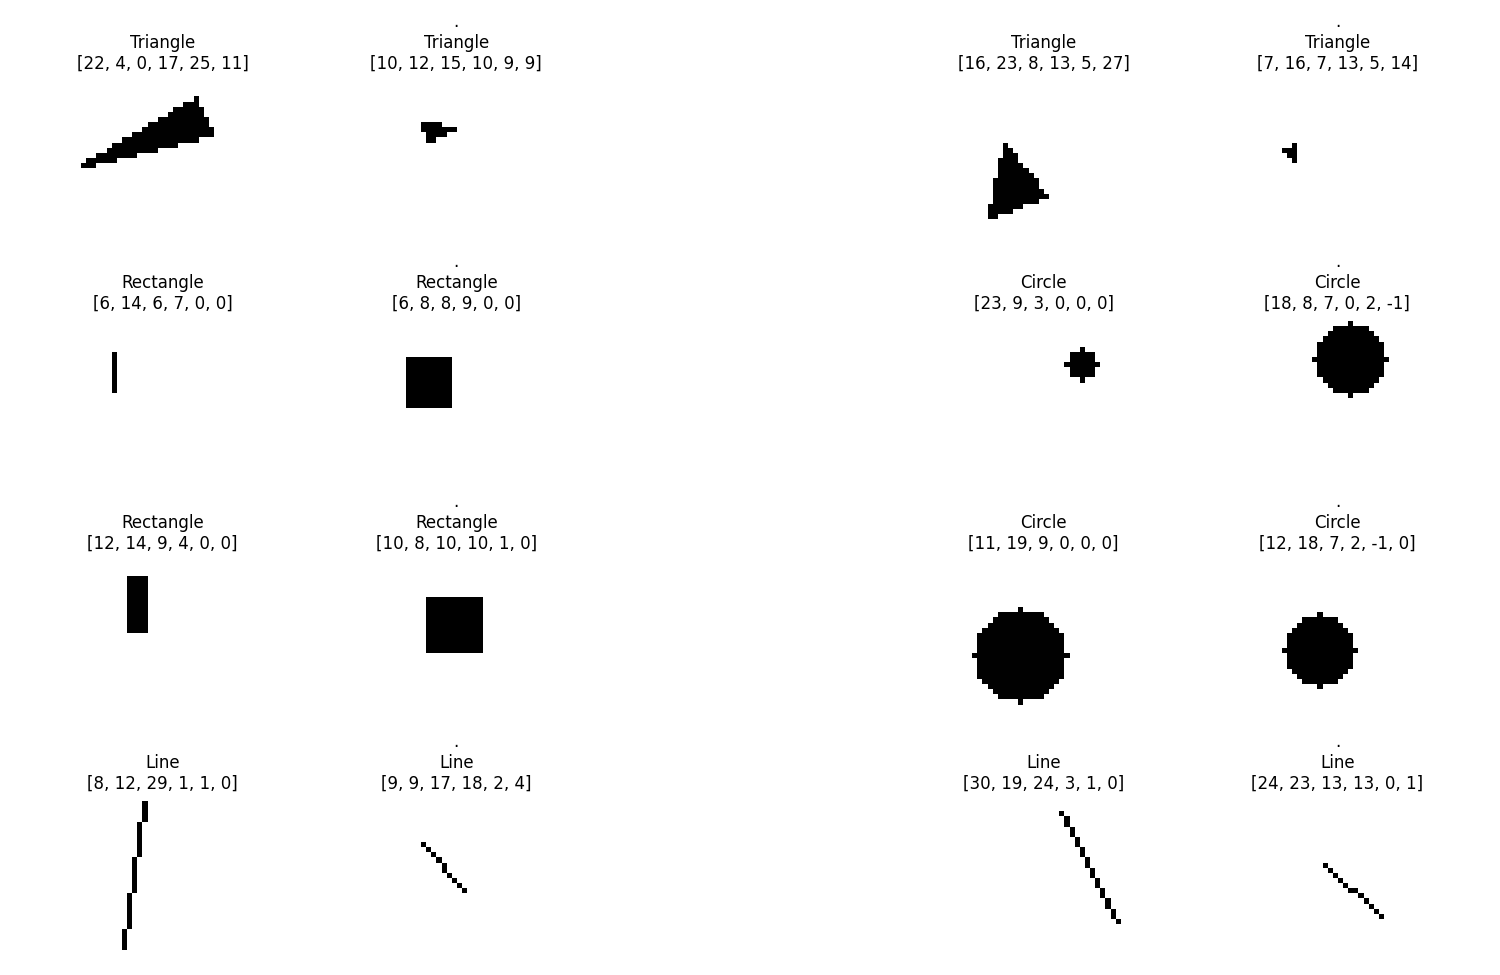
\includegraphics[width=1.0\textwidth]{../rc/images/all_shapes_approx_visual1.png}
    \vfill
    \begin{abstract}
		 This paper examines a particular approach for converting raster images with basic shapes into a vector representation.
		 It is demonstrated how a neural network can learn to extract the necessary data through training with on-the-fly generated data.
    \end{abstract}
\end{titlepage}


\chapter{Introduction}

Images have become an important part of everyday live. Most of which are stored digitally, thus making the search for effective storage of images an essential, well researched aspect of computer science.
Many different formats and compression have emerged, which can be categorized into two main categories - vector and raster formats.

\section{Vector and raster graphics}

Vector and raster graphics are two fundamentally different approaches on how to represent the content of an image, both of which have advantages in representing a certain kind of image. While raster images tend to store or approximate small parts of a given picture to approximate what it looks like, vector formats rather store a specification for what is displayed in an image, similar to how humans describe images.

Both methods have pros and cons, and are more appropriate for certain situations than others. Vector formats are ideal for images that are easily describable in shapes, especially those made up of one-colored areas. In such cases, vector graphics can describe those shapes more precise, without pixels, and are less storage intense. Raster formats in turn are better suited for images without easily distinguishable shapes, such as portraits or landcape images.

While format conversions among raster or vector formats and from vector to raster graphics can be done with a multitude of programs, the conversion from a raster image to a vector representation proves more challenging, especially because shapes have to be recognized.

Therefore a way to convert raster images into a vector format can be beneficial, and is not yet a solved problem.


\section{Existing approaches}

\section{Architecture of neural networks}

Deep neural networks can be structured in different ways, leading to different kinds of traits that are beneficial in certain situations over others. For raster to vector conversion following architectures are interesting.

\subsection{Convolutional neural network}

A convolutional neural network (CNN) is a type of neural network that uses a convolutional layer to extract features from an input image. It is useful to reduce the information of the single pixels to a sequence of single features, that fully connected layers then can learn to connect. In order to extract the relevant features, it uses different \emph{kernels}, which are moved through the images using a certain \emph{stride value}, and applied to the pixel values. The \emph{kernel} and \emph{stride} values can be used to reduce the information for the following layers directly. Alternatively after each convolution, a certain function can be applied, which reduces the processed features.

{
	\centering
	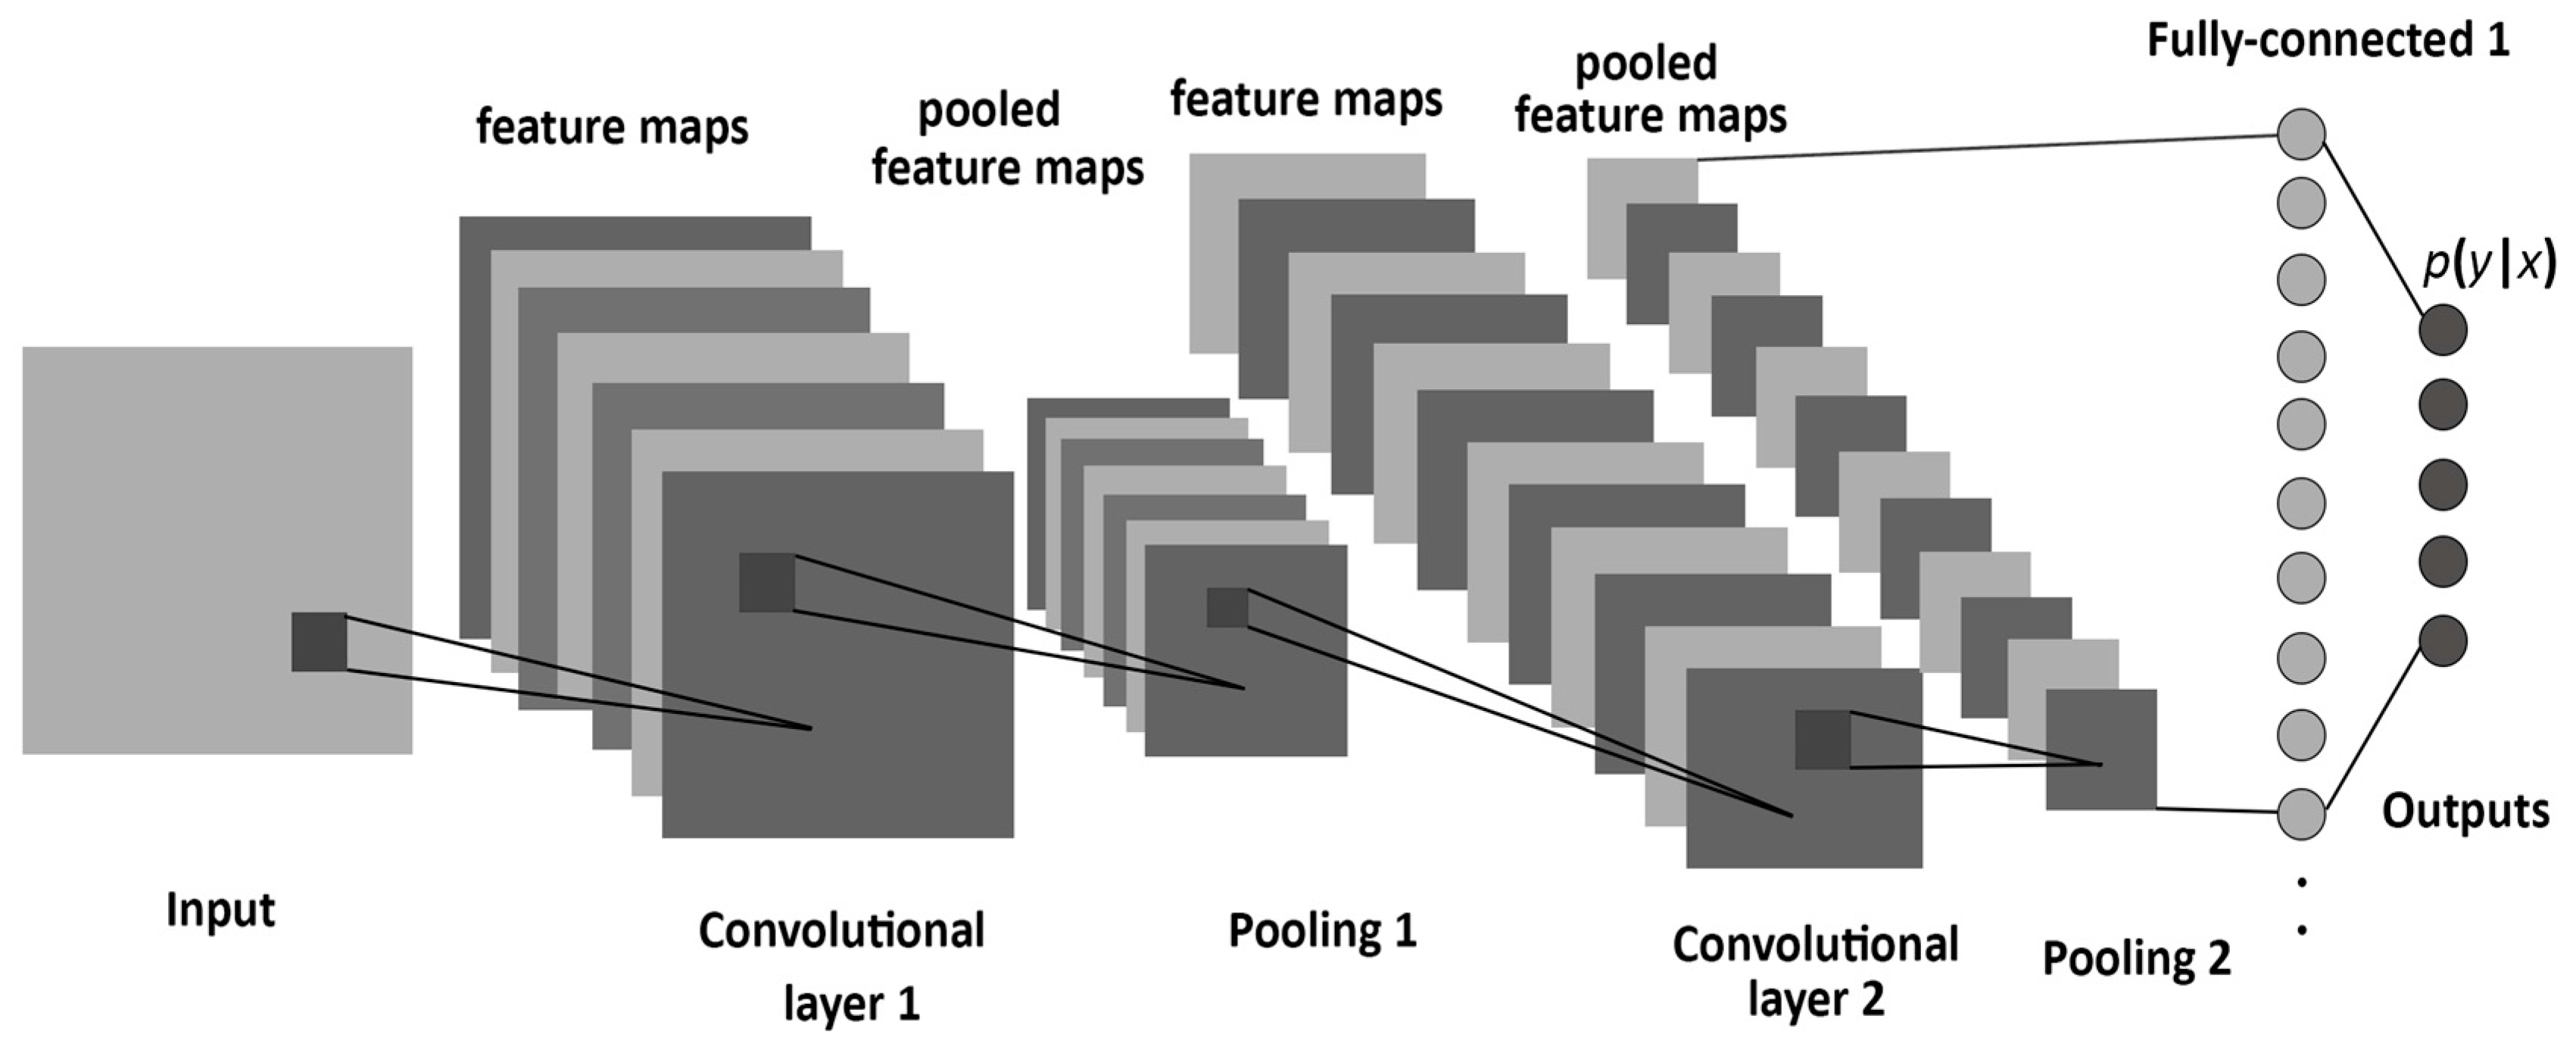
\includegraphics[width=0.5\textwidth]{../rc/images/cnn_architecture.png}
	\label{fig:cnn_architecture}
}


\subsection{Recurrent neural network}
\subsection{Reinforcement learning}


\chapter{Method}

\section{Overview}

The data 

\section{Framework choice}
\section{Language choice}



\section{Data generation}

The data that the model uses for training consists of raster images , with one shape in each of them. The images are internally represented as numpy arrays, where each entry represents the color values of a pixel. The background is white (i. e. RGB values set to (1, 1, 1)), and the pixels that fall within the shape are set to (0, 0, 0), thus appearing black, so that the contrast between shape and background is maximized.

All data generation is implemented in \lstinline{rtov/data/} and its subdirectories. A class, \lstinline{LazyDataset}, which inherits from the \lstinline{torch.utils.data.Dataset}, provides an interface, which a \lstinline{torch.utils.data.Dataloader} object can use later to get the next image. Therefore, the method \lstinline{__getitem__(self, i: int)} is provided, which loads a numpy array, draws a random shape on it and transforms it into a vector. Interesting is that the 

\section{Model architecture}

[TODO]

\section{Optimizing mechanisms}

[TODO]




\chapter{Discussion}

\section{Opportunities of generated training data for vectorization}

\section{Limits}

\section{Proposed model architectures}




\end{document}
